\documentclass[12pt,letterpaper]{article}
\usepackage[margin=15mm,headheight=16pt,headsep=7mm,footskip=9mm]{geometry}
\usepackage[T1]{fontenc}
\usepackage{lmodern}
\usepackage{tikz}
\usetikzlibrary{arrows.meta}
\usepackage{fancyhdr}
\usepackage{microtype}
\usepackage[hidelinks]{hyperref}
\pdfinfoomitdate=1
\pdftrailerid{}
\pdfsuppressptexinfo=15
\hypersetup{pdftitle={Week 80 Midnight laboratory - student materials},pdfauthor={Bellingham Math Circle}}
\setlength{\parindent}{0pt}
\setlength{\parskip}{7pt}
\pagestyle{fancy}
\fancyhf{}
\fancyhead[L]{\small Week 80 / Midnight laboratory / \band}
\fancyfoot[L]{\scriptsize Bellingham Math Circle / Week 80 / M80-D-v1}
\fancyfoot[R]{\scriptsize \thepage}
\renewcommand{\headrulewidth}{0.35pt}
\renewcommand{\footrulewidth}{0pt}
\newcommand{\band}{Grades 2--5}
\newcommand{\problem}[2]{\par\textbf{Problem #1:} #2\par}
\tikzset{every node/.style={font=\sffamily\small},line cap=round,line join=round}

% The two endpoint ticks on each full-width board are exactly 180 mm apart.
\newcommand{\timeline}[2]{%
\begin{tikzpicture}[x=1mm,y=1mm]
  \path[use as bounding box] (0,0) rectangle (184,44);
  \draw[line width=0.9pt] (2,19)--(182,19);
  \draw[line width=0.9pt] (2,15)--(2,23) (182,15)--(182,23);
  \node[anchor=west] at (2,7) {#1};
  \node[anchor=east] at (182,7) {#2};
\end{tikzpicture}}

\newcommand{\strip}[2]{%
\begin{tikzpicture}[x=1mm,y=1mm]
  \path[use as bounding box] (0,0) rectangle (184,38);
  \draw[dashed,gray,line width=0.5pt] (0,0) rectangle (184,36);
  \draw[line width=0.9pt] (2,21)--(182,21);
  \draw[line width=0.9pt] (2,17)--(2,25) (182,17)--(182,25);
  \node[anchor=west] at (2,7) {#1};
  \node[anchor=east] at (182,7) {#2};
\end{tikzpicture}}

\begin{document}
Start with the card OFF. The first switching mark is halfway from START to MIDNIGHT. Each next switching mark is halfway from the previous mark to MIDNIGHT. Flip the card at every switching mark. This rule keeps going before midnight.

\begin{center}
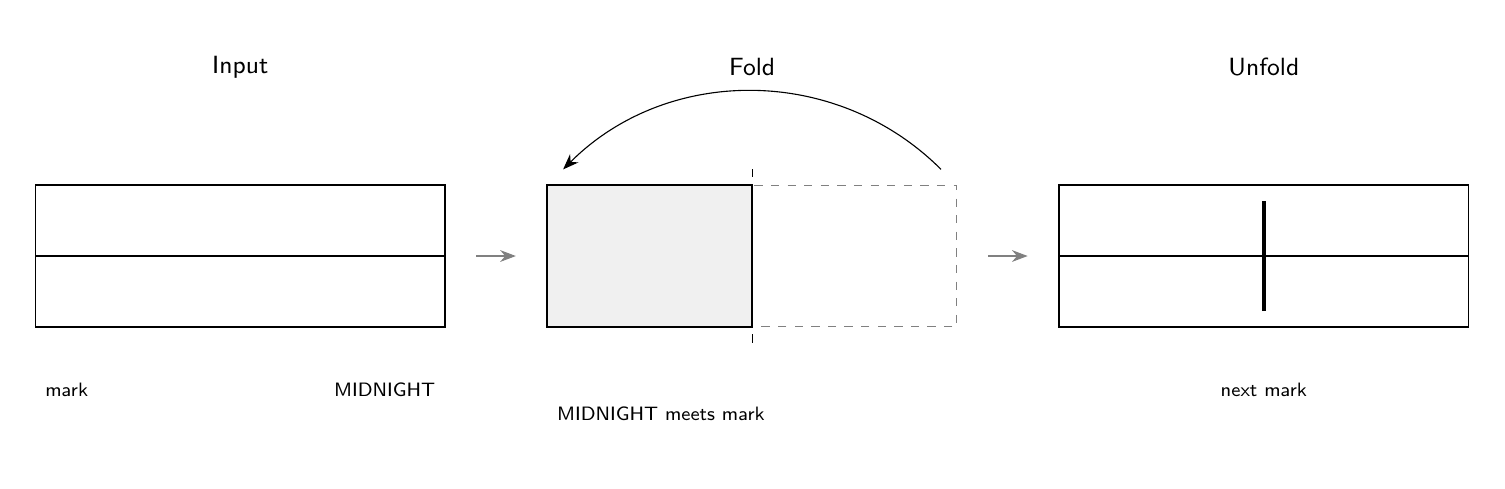
\begin{tikzpicture}[x=1mm,y=1mm]
  \path[use as bounding box] (0,-1) rectangle (184,54);
  % A single, non-task fold demonstrates how the remaining gap is halved.
  \node at (27,49) {Input};
  \draw[line width=0.6pt] (1,16) rectangle (53,34);
  \draw (1,25)--(53,25);
  \draw (1,22)--(1,28) (53,22)--(53,28);
  \node[anchor=west,font=\sffamily\scriptsize] at (1,8) {mark};
  \node[anchor=east,font=\sffamily\scriptsize] at (53,8) {MIDNIGHT};
  \draw[-{Stealth[length=2mm]},gray] (57,25)--(62,25);

  \node at (92,49) {Fold};
  \draw[dashed,gray] (66,16) rectangle (118,34);
  \draw[line width=0.8pt,fill=gray!12] (66,16) rectangle (92,34);
  \draw[dashed] (92,14)--(92,36);
  \draw[-{Stealth[length=2mm]}] (116,36) to[out=135,in=45] (68,36);
  \node[anchor=west,font=\sffamily\scriptsize,align=left] at (66,5) {MIDNIGHT\ meets mark};
  \draw[-{Stealth[length=2mm]},gray] (122,25)--(127,25);

  \node at (157,49) {Unfold};
  \draw[line width=0.6pt] (131,16) rectangle (183,34);
  \draw (131,25)--(183,25);
  \draw (131,22)--(131,28) (183,22)--(183,28);
  \draw[line width=1.2pt] (157,18)--(157,32);
  \node[font=\sffamily\scriptsize] at (157,8) {next mark};
\end{tikzpicture}
\end{center}

\problem{1}{Make the first four switching marks on a paper strip. Play the rule with the card. Can the rule have a last switching mark before midnight?}

\begin{center}\timeline{START}{MIDNIGHT}\end{center}
\vfill
\newpage

\problem{2}{Use the same switching marks. The card starts OFF. A counter starts at START. At each switching mark, flip the card and move the counter halfway from its present place toward END. As the rule keeps going, does the card settle on one side? What place does the counter approach?}

\begin{center}
\begin{tikzpicture}[x=1mm,y=1mm]
  \path[use as bounding box] (0,0) rectangle (184,53);
  \draw[line width=0.9pt] (2,23)--(182,23);
  \draw[line width=0.9pt] (2,19)--(2,27) (182,19)--(182,27);
  \draw[line width=0.8pt,fill=white] (2,23) circle (3);
  \node[anchor=west] at (2,8) {START};
  \node[anchor=east] at (182,8) {END};
\end{tikzpicture}
\end{center}

\vspace{12mm}
\begin{center}
\begin{tikzpicture}[x=1mm,y=1mm]
  \path[use as bounding box] (0,0) rectangle (184,109);
  \node[anchor=west] at (2,103) {Card};
  \node[anchor=west] at (98,103) {Counter};
  \draw[gray!50] (92,0)--(92,106);
\end{tikzpicture}
\end{center}
\vfill
\newpage
\renewcommand{\band}{Grades 4--5}

\problem{3}{What, if anything, does the switching rule alone tell you to show at midnight? Use the card and switching marks to support your answer.}

\vspace{10mm}
\begin{center}\timeline{START}{MIDNIGHT}\end{center}

\vspace{15mm}
\begin{center}
\begin{tikzpicture}[x=1mm,y=1mm]
  \path[use as bounding box] (0,0) rectangle (184,76);
  \draw[rounded corners=2mm,line width=0.7pt] (59,12) rectangle (125,65);
  \node at (92,70) {MIDNIGHT};
\end{tikzpicture}
\end{center}
\vfill
\newpage

\problem{4}{Keep every switch before midnight. Make two different extra rules for the card at midnight. Decide whether either extra rule follows from the original switching rule.}

\vspace{6mm}
\begin{center}
\begin{tikzpicture}[x=1mm,y=1mm]
  \path[use as bounding box] (0,0) rectangle (184,54);
  \draw[line width=0.6pt] (1,0) rectangle (88,52);
  \draw[line width=0.6pt] (96,0) rectangle (183,52);
  \node[anchor=north west] at (4,49) {At midnight:};
  \node[anchor=north west] at (99,49) {At midnight:};
\end{tikzpicture}
\end{center}

\vspace{13mm}
\problem{5}{Someone adds this rule: ``At midnight, use the state that the earlier states approach.'' Try that rule for the ON/OFF card and for the moving counter. Does it assign a state in each case?}
\vfill
\newpage
\renewcommand{\band}{Grades 2--5}

\begin{center}
\strip{START}{MIDNIGHT}

\vspace{11mm}
\strip{START}{END}

\vspace{23mm}
\begin{tikzpicture}[x=1mm,y=1mm]
  \path[use as bounding box] (0,0) rectangle (184,57);
  \draw[dashed,line width=0.6pt] (12,0) rectangle (88,54);
  \draw[dashed,line width=0.6pt] (96,0) rectangle (172,54);
  \node[font=\sffamily\bfseries\fontsize{32}{36}\selectfont] at (50,27) {ON};
  \node[font=\sffamily\bfseries\fontsize{32}{36}\selectfont] at (134,27) {OFF};
\end{tikzpicture}
\end{center}
\vfill
\end{document}
